% Results are preserved in Question 2 - Leaderboard/results/ and submission_snapshots/.
\section{Task 2: Leaderboard Challenge}

\subsection{Data and forecasting setup}
The task is to forecast 168 values of an anonymised, non-negative physical quantity
from 43\,656 observed values. The original units, dates and identity are unavailable.
Ten optional external variables cover both the history and forecast horizon;
using their future values is explicitly permitted.
\begin{itemize}
  \item \textbf{Short memory and heavy tails.} Target autocorrelation is 0.97 at lag 1,
        0.40 at lag 24 and about 0.02 by lag 96. The median is 73, the 99th percentile
        418 and the maximum 994. Persistence alone is therefore unlikely to forecast
        the whole horizon well, and missing a few large peaks can dominate RMSE.
  \item \textbf{Recovered periodicity.} The spectrum and autocorrelation show a
        24-step cycle. I use index-derived sine/cosine features with periods 24 and
        8\,766. Interpreting these as daily and yearly cycles is an assumption,
        not something the anonymised timestamps establish.
  \item \textbf{Processing.} The target and continuous inputs are globally
        standardised using only the fit region. The non-negative variables D, E and F
        use $\log(1+x)$. Inputs include the ten optional variables, their trailing
        6- and 24-step means, and origin-relative marks ($h/168$ and $e^{-h/24}$).
        Trailing features use external data only; no future target enters an input.
\end{itemize}

\subsection{Chronological validation}
\begin{itemize}
  \item \textbf{Development split.} Fit on $[0,26304)$, early-stop on
        $[26304,35064)$ (origins every 24 steps), and compare designs on
        $[35088,43656)$: \textbf{51 non-overlapping 168-step blocks}.
        All blocks start at the same phase of the 24-step cycle as the hidden horizon.
  \item \textbf{Multiple seeds.} Each development configuration uses three seeds.
        Tables report seed mean and standard deviation unless identified as ensemble
        results. Paired block comparisons use the seed-averaged block errors.
        Seed spread is comparable to many design gains, so single runs are insufficient.
  \item \textbf{Second fold.} Later comparisons also fit on $[0,17520)$,
        early-stop on $[17520,26304)$ and evaluate the next 52 weekly blocks.
        The 16 edge weeks of the recent fold and 17 of the earlier fold are called
        \emph{winter-like} below, based on the assumed yearly cycle. Their errors are
        a useful stress test, but the season and hidden-week difficulty are uncertain.
  \item \textbf{Selection.} The first submission used full-holdout RMSE, with cost
        and edge-week performance as tie-breakers. Later changes were checked on both
        folds, seeking a mean weekly edge-error reduction of at least 3 RMSE and wins
        on at least 20 of 33 edge weeks. These development periods were reused during
        model selection, so they are not an untouched final test.
\end{itemize}

\subsection{Autoformer and initial design choices}
The encoder-decoder is written in \path{pa1q2/autoformer.py}.
It follows Wu et al. (2021), the public \path{thuml/Autoformer} implementation, and the delay-aggregation
convention from Task 1. It contains both required mechanisms:
\begin{itemize}
  \item \textbf{Progressive decomposition.} A centred moving average (kernel 25,
        replicate padding) separates trend and residual at the input and after every
        sublayer. Decoder trend contributions are accumulated through a projection.
  \item \textbf{Auto-Correlation.} FFT-based scores from learned queries and keys
        select $k=\lfloor\ln L\rfloor$ delays, followed by softmax-weighted circular
        aggregation of values. This replaces pointwise attention in encoder self,
        decoder self and decoder cross mixing.
  \item \textbf{Initial training.} Context 168, label length 48, horizon 168, one
        encoder and decoder layer, four heads, dropout 0.1, batch 64, gradient clip 1,
        MSE on the standardised raw target. Adam starts at $3\cdot10^{-4}$, halves
        each epoch, and stops with patience 2, at most six epochs. Final-model changes
        are specified in Section~\ref{sec:final}.
\end{itemize}

\subsection{Required optional-data ablation}
Three seeds per configuration, $d_\text{model}=32$; ES is early-stopping RMSE and
holdout covers 51 recent blocks.
\begin{center}\small
\begin{tabular}{lrrrrrr}
\toprule
Optional inputs & Params & ES RMSE & Holdout RMSE & MAE & sMAPE (\%) & Edge RMSE\\
\midrule
None                  & 21\,569 & 102.6 & 97.7 $\pm$ 2.8 & 72.2 & 74.9 & 119.4\\
Past only             & 27\,329 & 104.9 & 99.0 $\pm$ 0.9 & 72.2 & 78.6 & 119.9\\
Past + horizon        & 23\,489 & 79.2  & 74.4 $\pm$ 1.3 & 51.7 & 72.8 & 88.2\\
\bottomrule
\end{tabular}
\end{center}
Reference holdout RMSEs are
climatology 93.0, last-week mean 97.9, persistence 147.7, direct ridge without
covariates 87.7, and direct ridge with known-horizon covariates 71.5.
\begin{itemize}
  \item \textbf{Horizon values matter.} Known-horizon inputs reduce RMSE by 24\%
        (97.7 to 74.4), improve MAE and sMAPE, and beat the no-input model on 44 of 51
        blocks (paired sign test $p\approx10^{-7}$). The effect is much larger than
        the seed spread. External conditions during the forecast horizon carry useful
        information beyond the target history.
  \item \textbf{Past-only inputs did not help here.} Their 99.0 RMSE is close to
        97.7 without external data. This supports feeding the known horizon to the
        decoder, rather than relying on encoder history alone; it is not a claim that
        past covariates are generally useless.
\end{itemize}

\begin{figure}[h]\centering
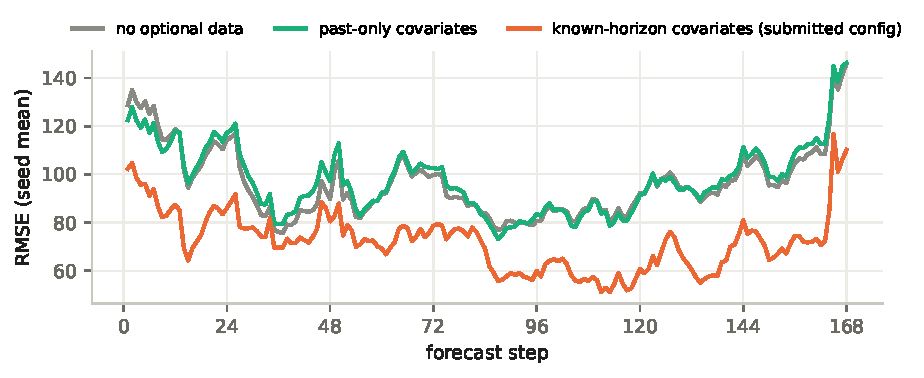
\includegraphics[width=0.49\linewidth]{figures/q2_horizon.pdf}\hfill
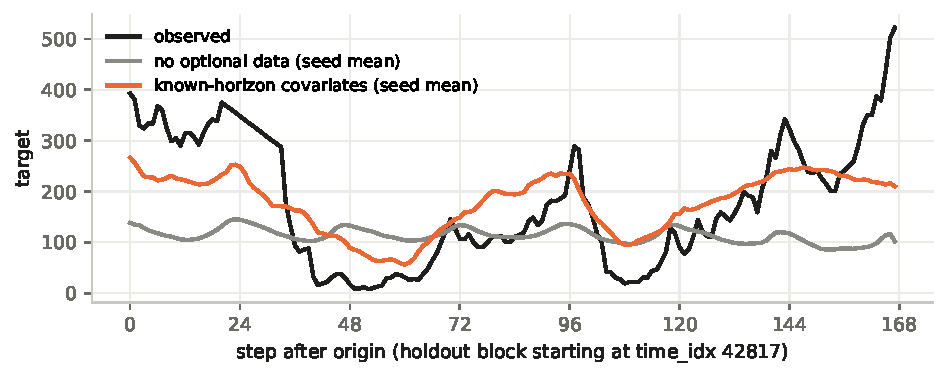
\includegraphics[width=0.49\linewidth]{figures/q2_example_week.pdf}
\caption{Left: per-step holdout RMSE (seed mean); the known-horizon model improves
every step. Right: an example from the most volatile late-year holdout week.}
\label{fig:q2horizon}
\end{figure}

\subsection{Which changes were worth keeping?}
\begin{center}\small
\begin{tabular}{lrrr}
\toprule
Initial variant (known-horizon inputs, three seeds) & Params & Holdout RMSE & Edge RMSE\\
\midrule
$d=32$ base                         & 23\,489 & 74.4 $\pm$ 1.3 & 88.2\\
$d=32$, $\log(1+y)$ target          & 23\,489 & 81.6 $\pm$ 10.4 & 88.2\\
$d=16$                              & 6\,625  & 75.1 $\pm$ 1.1 & 87.1\\
$d=16$, width-5 input embedding     & 10\,977 & 74.5 $\pm$ 2.6 & 85.5\\
\quad + horizon marks, no anchor   & 11\,297 & 73.2 $\pm$ 2.4 & 82.9\\
\quad + horizon marks and anchor   & 11\,297 & 72.9 $\pm$ 1.9 & 85.4\\
\bottomrule
\end{tabular}
\end{center}
\begin{itemize}
  \item \textbf{Raw target and a small model.} Log-target training improved MAE and
        sMAPE but under-predicted large peaks and gave unstable RMSE. Halving model
        width cost little measurable accuracy, so $d=16$ was preferable under the
        parameter/epoch penalty. More parameters or epochs alone did not establish
        a better model.
  \item \textbf{Horizon marks.} Origin-relative features explicitly identify the
        forecast step. Together with replicate padding they improved boundary errors
        and holdout RMSE. Anchoring was a close comparison (72.9 versus 73.2), so the
        anchored configuration was used for attempt 1, rather than claimed as a
        decisive improvement.
  \item \textbf{Negative results.} Refitting on more history, wider decomposition,
        extra rolling features, winter-weighted loss and square-root targets did not
        consistently improve edge weeks. A 27-model mixture improved recent-fold
        RMSE only from 69.3 to 68.1, at $P=345\,435$, $E=122$; it was not submitted.
        Full records remain in the repository.
\end{itemize}

\textbf{A more direct path for horizon inputs.} A covariate-only gradient-boosting
baseline scored 57.0 overall and 70.5 on recent edge weeks, against 69.3 and 82.0 for
the attempt-1 ensemble. This suggested that the horizon inputs held signal the
sequence model was not fully using. One possible explanation is smoothing inside
the decomposition/mixing path, but this mechanism was not isolated experimentally.
I compared a nonlinear covariate embedding with an additive per-step covariate head:
\begin{center}\small
\begin{tabular}{llrrr}
\toprule
Fold & Three-seed ensemble & All-week RMSE & Edge RMSE & Edge weeks won\\
\midrule
Recent  & Attempt-1 configuration & 69.34 & 81.97 & --\\
        & Covariate embedding MLP & 64.79 & 76.80 & 8/16\\
        & Direct covariate head   & 61.68 & 74.97 & 12/16\\
Earlier & Attempt-1 configuration & 77.43 & 106.13 & --\\
        & Covariate embedding MLP & 74.36 & 102.48 & 12/17\\
        & Direct covariate head   & 66.40 & 91.63 & 12/17\\
\bottomrule
\end{tabular}
\end{center}
Wins are relative to attempt 1 on the same blocks. The direct-head configuration
reduced mean weekly edge RMSE by 8.3 and won 24 of 33 weeks across both folds.
It also removes anchoring and changes the learning-rate schedule; these results
support the combined configuration, not the head's isolated contribution.

\subsection{Leaderboard results}
\begin{center}\small
\begin{tabular}{clrrrrr}
\toprule
Attempt & Model (three members) & RMSE & MAE & sMAPE (\%) & $P$ & $E$\\
\midrule
1 & Anchored Autoformer     & 81.56 & 60.96 & 57.81 & 33\,891 & 15\\
2 & Covariate embedding MLP & 81.93 & 62.75 & 59.58 & 38\,979 & 16\\
3 & Direct covariate head   & \textbf{62.95} & \textbf{46.31} & \textbf{49.63} & 53\,670 & 20\\
\bottomrule
\end{tabular}
\end{center}
\begin{itemize}
  \item Attempt 1 ranked fourth when submitted. Its 69.34 historical ensemble RMSE
        did not predict the hidden-week result. Edge-week RMSE of 81.97 was closer,
        consistent with seasonal difficulty, but neither estimate guarantees a rank.
  \item Attempt 2 improved historical validation in both folds but did not improve
        the scored week. A single 168-step block can disagree with a multi-block
        estimate, especially for a heavy-tailed series.
  \item Attempt 3 scored 62.96 after the efficiency penalty and ranked first at the
        time (previous best 69.16). RMSE was 23\% below attempt 1. This is a reported
        result, not a guarantee about later rankings or other weeks. Leaderboard
        feedback prompted further historical checks; candidate selection used those
        checks and early stopping, not access to hidden targets.
\end{itemize}

\subsection{Final submitted model (attempt 3)}\label{sec:final}
\begin{itemize}
  \item \textbf{Architecture.} Autoformer with $L=168$, label length 48,
        \texttt{pred\_len}=168, one encoder and decoder layer, $d_\text{model}=16$,
        four heads, $d_\text{ff}=32$, kernel 25, dropout 0.1, width-5 covariate
        embedding, replicate padding and horizon marks. A direct head
        ($36\to64\to64\to1$, GELU) maps each step's known inputs to an additive
        forecast correction. Decomposition and all three Auto-Correlation mixers
        remain present. There is no last-value anchoring.
  \item \textbf{Training and selection.} Fit on $[0,35064)$ and early-stop on the
        51 recent blocks, with Adam at $10^{-3}$ decayed by 0.8 per epoch, patience 3,
        at most ten epochs, batch 64, MSE and gradient clip 1. Of seven seeds (0--6),
        seeds 2, 3 and 4 form the final ensemble, selected using the early-stopping
        set. Their best RMSEs are 59.7, 65.8 and 63.7, at epochs 4, 4 and 3.
        Seeds 0, 1 and 6 stopped at RMSE 81--83; seed 5 was also excluded to keep
        the ensemble at three members. Selection adds uncertainty beyond an
        unselected three-seed comparison.
  \item \textbf{Forecast and cost.} Each member's forecast is floored at 7.0 (the
        fit-region target's 1st percentile), then the three forecasts are averaged.
        The 168 outputs cover \texttt{time\_idx} 43\,657--43\,824 in order.
        $P=3\times17\,890=53\,670$ and $E=7+7+6=20$, including patience epochs;
        there was no full-history refit. Four discarded runs used a further 17 epochs,
        disclosed here but excluded from the submitted members' total.
  \item \textbf{Reproduction.} The \path{submission/} folder holds the forecasts
        and declaration. The declaration records all member arguments and epoch counts.
        \texttt{pa1q2.submission} reloads weights and checks parameter counts.
        Training/export commands are in the Task 2 README. Final snapshot:\\
        \path{submission_snapshots/covhead_s2_s3_s4_2026-09-29/}.
\end{itemize}

\textbf{Limits and takeaway.} The final comparison changes the covariate head,
anchoring and schedule together. It does not prove that smoothing caused the earlier
errors. Development blocks were reused, the final members were selected on early
stopping, and the hidden score covers only one week. The strongest finding is the
large benefit of known-horizon inputs in the required multi-seed ablation. The final
configuration makes better use of those inputs while keeping the Autoformer mechanisms.

\clearpage
\begin{figure}[ht]\centering
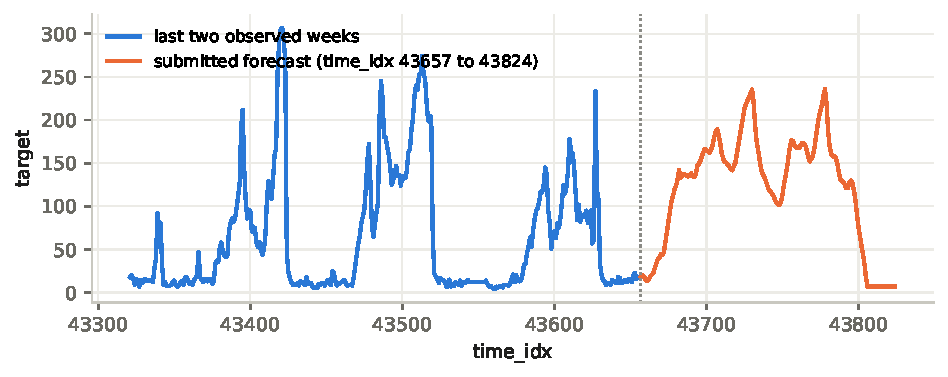
\includegraphics[width=0.74\linewidth]{figures/q2_final_forecast.pdf}\\[4pt]
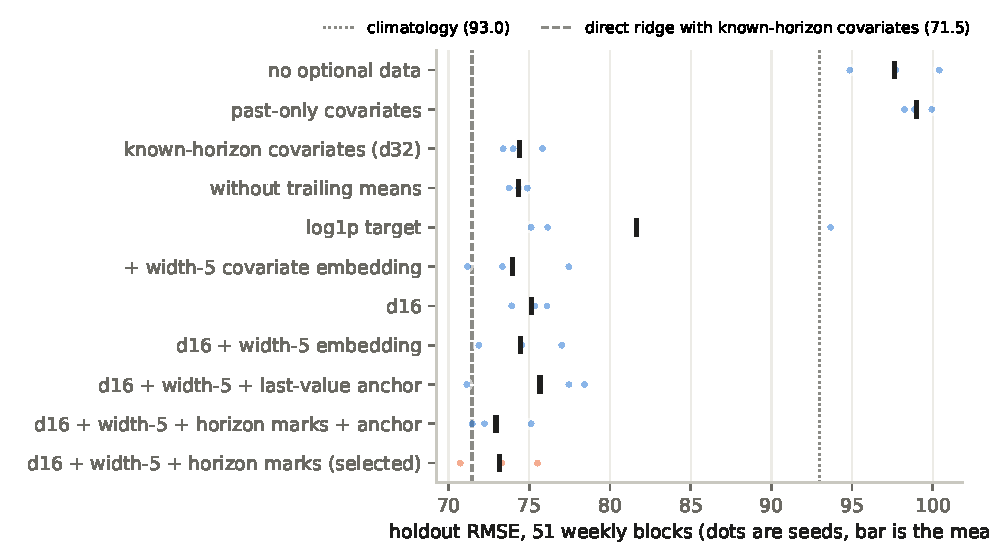
\includegraphics[width=0.95\linewidth]{figures/q2_ablation.pdf}
\caption{Top: last two observed weeks and the attempt-3 forecast. Bottom: initial
ablation runs on 51 holdout blocks (dots are seeds, bars are means); reference lines
show climatology and covariate ridge. The initial selected row refers to attempt 1.}
\label{fig:q2final}
\end{figure}

\subsection{Short reflections}
The direct 168-step output avoids feeding forecast errors back into the model,
although horizon errors can remain correlated. Global scaling preserves absolute
level; restoring a window's level after relative normalisation would not by itself
let the network condition on that level. Known-horizon inputs belong in the forecast
path, as the optional-data ablation demonstrates. Integer indices allow recovered
phase features on this regular grid, but they do not establish weekdays, holidays
or a real calendar; the yearly interpretation remains an assumption.
